% <<<<<< Rapport projet de troisième année >>>>>>

\documentclass[a4paper,12pt,titlepage]{report}
\usepackage[utf8]{inputenc}
\usepackage[T1]{fontenc}
\usepackage{lmodern}
\usepackage[a4paper]{geometry}
\usepackage[french]{babel}
\usepackage{amsmath}
\usepackage{amssymb}
\usepackage{mathrsfs}

\usepackage{graphicx}
\usepackage{appendix}
\usepackage{hyperref}
\usepackage{subcaption}
\usepackage{setspace}
\usepackage[intoc]{nomencl}
%\usepackage{algorithm}
%\usepackage{listing}
\usepackage{verbatim}

\begin{document}


%==================================== Page de Garde ==============================
\begin{titlepage}
 
	\begin{center}
	\begin{figure}[!h]
	\centering	
		\begin{subfigure}[b]{0.3\textwidth}
		
\includegraphics[height = 2cm, keepaspectratio]{graphes/mines_nancy.png}
		\end{subfigure}
		\begin{subfigure}[b]{0.3\textwidth}
		
\includegraphics[height = 2cm, keepaspectratio]{graphes/elie_cartan.png}
		\end{subfigure}
		\begin{subfigure}[b]{0.3\textwidth}
		
\includegraphics[height = 2cm, keepaspectratio]{graphes/univ_lorraine.png}
	\end{subfigure}
	\end{figure}
 
	\textsc{École nationale supérieure des Mines de Nancy}\\[2cm]
	\textsc{Rapport de projet 3A}\\[1cm]
	\textsc{Pierre Gauthier}\\[1cm]
 
	\begin{doublespace}
		{ \huge \bfseries{Algorithme d'apprentissage en chimie quantique et application au screening (sélection) de cellules photovoltaïques}}\\[2cm]
	\end{doublespace}
	\textmd{Laboratoire : Institut Élie Cartan}\\[1cm]
	\textmd{Tuteurs : Dario Rocca et Marianne Clausel}
	% Bottom of the page
	\vfill
	{\textit{{\large 21 Novembre 2018}}}
 
	\end{center}
\end{titlepage}

%================= Table des matières ===============================
\tableofcontents

\newpage



%======================== Introduction ==============================
\textbf{\Huge Introduction:} \\
\newline

Ce projet est conduit dans un cadre pédagogique en tant que projet de troisième année à l'Ecole des Mines de Nancy. Il suit la publication scientifique de Mathias Rupp "Machine Learning for Quantum Mechanics in a Nutshell". Dans cette publication Mathias Rupp propose d'allier la mécanique quantique aux méthodes de machines learning pour faire de la prédiction à partir de données et ainsi dépasser les problèmes en terme de puissance de calcul du problème à N-corps. Il vise ainsi à prédire l'énergie d'atomisation de molécules à partir d'un set de données d'entrainement, en utilisant des méthode de  linéaire, notamment la régression à vecteur supports (SVM). 
Le premier objectif du projet est de reproduire les résultats de cette études, et d'explorer des variations dans les paramètres sur l'erreur finale de prédiction. Nous pourrons également dépasser le travail réaliser dans l'étude en travaillant sur des données avec de nouveaux descripteurs qui prennent en compte les propriétés des groupes chimiques des molécules.\\
Nous allons dans une première partie présenterer les méthodes à vecteur support avec l'astuce des noyaux.

\chapter{Support Vector Machines methods (SVM)}

Le probléme SVM vise à séparer les données $(x_{i},\ y_{i})_{1 \leqslant i \leqslant N},\ x_{i} \in \mathbb{R}, \ y_{i} \in \{-1,\ 1\}$ en deux classes $+1$ et $-1$ à l'aide de la fonction $f(x) = w \cdot x + b \ (b \in \mathbb{R},\ w \in  \mathbb{R}^{d})$ telle que $f(x) > 0 \Rightarrow x \in C_{+1}$, et $f(x) < 0 \Rightarrow x \in C_{-1}$

\begin{figure}[!h]
	\begin{center}
	\centering	
	%\begin{subfigure}[b]{0.3\textwidth}
		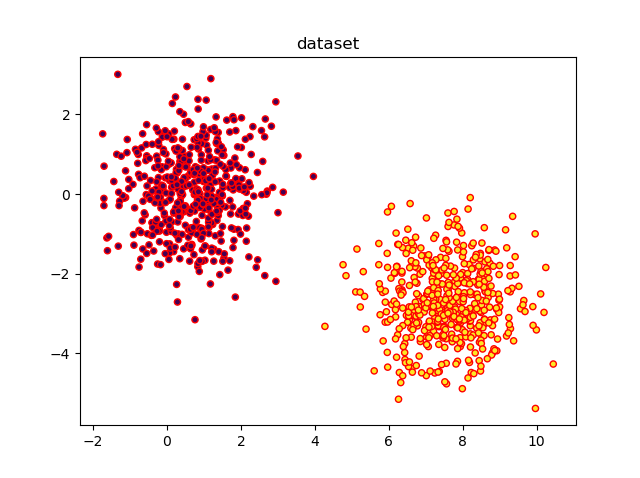
\includegraphics[height = 5cm, keepaspectratio]{graphes/SVM_donnee.png}
		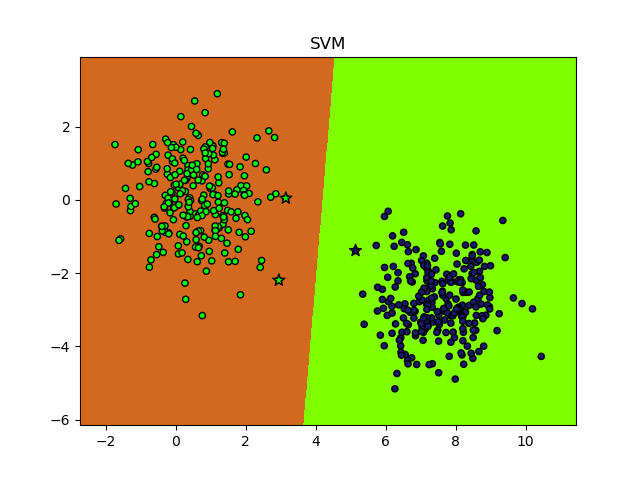
\includegraphics[height = 5cm, keepaspectratio]{graphes/SVM_separee.png}
		\caption{sparation de données générées make$\_$blobs du package dataset et séparation de l'espace en deux classe par la méthode des vecteurs support à l'aide de la fonction SVC du package sklearn. Les étoiles sont les vecteurs supports.}
			%\end{subfigure}
	\end{center}
\end{figure}
Nous voulons trouver l'hyperplan qui sépare le mieux nos données parmi tous ceux compatibles.

Pour juger la qualité d’un hyperplan en tant que séparateur on utilise la distance entre les exemples d’apprentissage et ce séparateur. Plus précisément, la « marge » d’un problème d’apprentissage est définie comme la distance entre le plus proche exemple d’apprentissage et l’hyperplan de séparation. \\
Pour un hyperplan $H$, On a :
\[
\text{Marge}(H) = \text{min}_{x_{i}}\ d(x_i,\ H)
\]
\begin{figure}[!h]
	\begin{center}
	\centering	
	%\begin{subfigure}[b]{0.3\textwidth}
		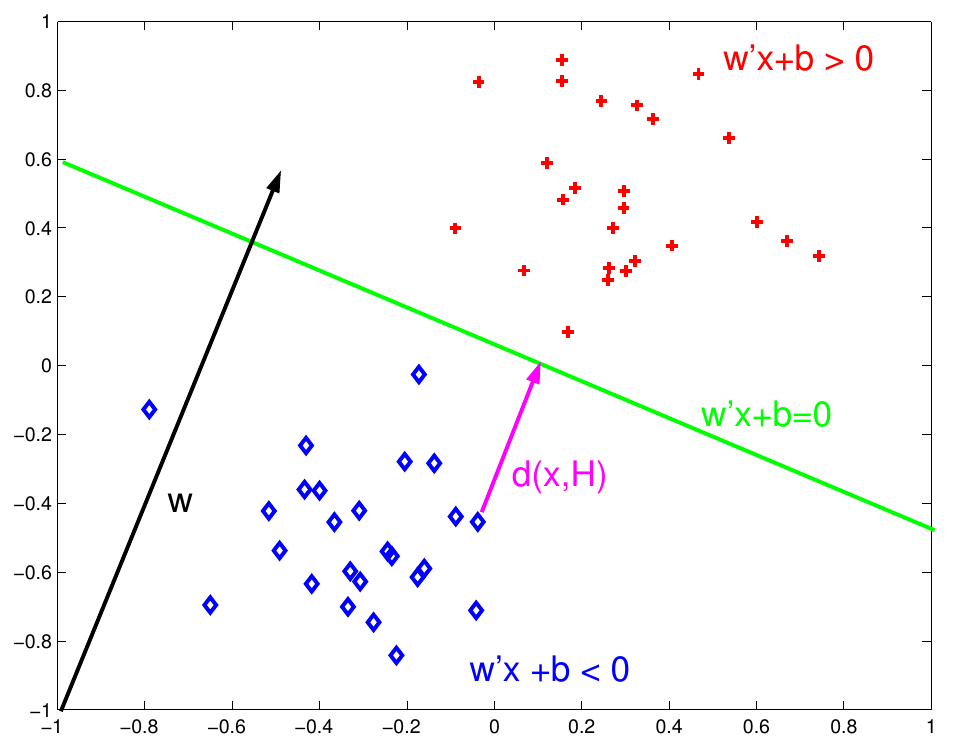
\includegraphics[height =6cm, keepaspectratio]{graphes/svm05.png}
		\caption{Le séparateur idéal correspond intuitivement à l’hyperplan qui passe « au milieu » entre les données sans préférence pour une classe ou une autre. C’est le séparateur de marge maximale.[Cours Cnam RCP209]}
			%\end{subfigure}
	\end{center}

Sous l'hypothèse qu'il exixte un hyperplan qui sépare nos données, trouver l'hyperplan qui maximise la marge revient à résoudre le problème suivant:
\[
	\left\{
	\begin{array}{ccc}		
	\begin{aligned}
		&\text{arg}\ \text{min}_{w,b}\ \frac{1}{2}||w||^{2} \\
		&\forall \ 1 \leqslant i \leqslant N,\ y_i (w \cdot x_i + b)\geqslant 1
	\end{aligned}
\end{array}
	\right.
% − \sum{ \lambda_{i} (y_{i} (w \cdot x_i + b)−1)}
\]

On utilise le lagrangien des conditions de Karush, Kuhn et Tucker, qui s'exprime sous la forme suivante :
\[
L(w,b,\lambda_{i}) = \frac{1}{2}||w||^{2} - \sum{\lambda_{i}( y_i (w \cdot x_i + b)-1)}
\]

On recherche donc le $\lambda$ qui maximise
\[
\text{max}\ L(\lambda) = \sum_{i}{\lambda_{i}} - \frac{1}{2} \sum_{i}{\sum_{j}{\lambda_{i} \lambda_{j} y_i y_j x_i \cdot x_j}} 
\]
\[
\text{sous contraintes}\ \lambda_i \geqslant 0 \  \text{et} \sum_{i}\lambda_i y_i = 0 
\]
\end{figure}

On utilise alors l'astuce du noyaux qui consiste à remplacer le produit scalaire $x \cdot y$
par un noyaux reproduisant $K(x,y) = \phi(x) \cdot \phi(y)$, $K :\xi \time \xi \rightarrow \mathbb{R}$, $\phi :\xi \rightarrow \mathbb{R}$  . Le théorème de Mercer assure l'existence d'une telle décomposition du noyaux $K$

\begin{figure}[!h]
	%\begin{center}
		
	%\begin{subfigure}[b]{0.3\textwidth}
		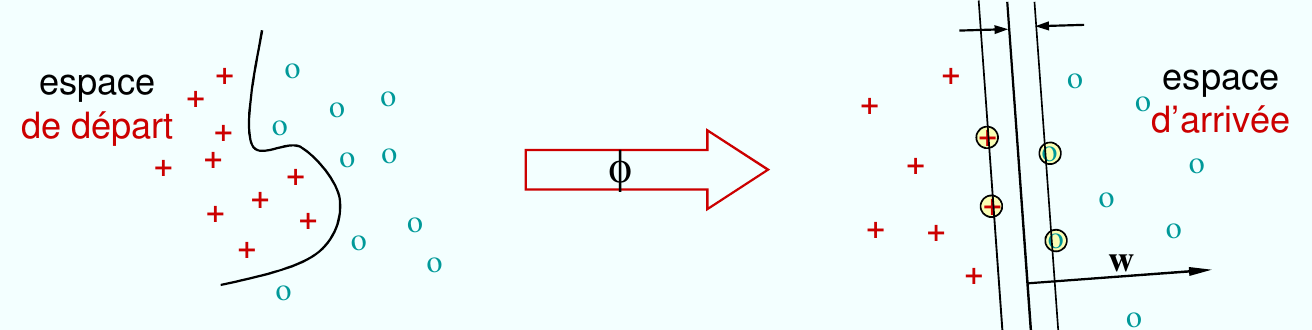
\includegraphics[height = 4cm, keepaspectratio]{graphes/mnoyaux05.png}
		\caption{Astuce à noyaux : projeter les données dans un espace de dimension beaucoup plus grande, où elles deviennent séparables linéairement.[Cours Cnam RCP209]}
			%\end{subfigure}
	%\end{center}
\end{figure}

\chapter{Experimentations}

test synchro overleaf
\end{document}
